\documentclass[12pt]{article}
\usepackage{graphicx}
\usepackage{multirow}
\usepackage{amsmath}
\usepackage{fullpage}
\usepackage{times}
\setlength\parindent{0pt}
\setlength\parskip{12pt}

\begin{document}

{\sffamily
\begin{tabular}{ll}
\multirow{3}{*}{\includegraphics[width=1in]{ach.png}}\\
& \Large{\em CONFIDENTIAL COMMITTEE MATERIALS} \\
&\\
& \textbf{\Huge{SIGBOVIK 2017 Paper Review}} \\
&\\
& \LARGE{Paper 75: RRR for UUU: Exact Analysis of Pee}\\
& \LARGE{Queue Systems with Perfect Urinal Etiquette} \\
&\\
\hline
\end{tabular}}
\vspace{2em}
\thispagestyle{empty}

{\large\bf
\begin{tabular}{l}
I. P. Freeley, Low-brow humor expert\\
Rating: X\\
Confidence: Shaky\\
\end{tabular}}
\vspace{1em}

This very detailed and well-researched paper promises to raise the state of
the art in SIGBOVIK bathroom humor. I was unable to evaluate the technical
contribution because, after many years as a SIGBOVIK reviewer, I am unaccustomed
to seeing real math. However, there were a number of avenues of research
which were not discussed in the paper, which could make the submission more
complete or at least be valuable considerations for future work. For example,
the paper considers only the discrete case. I wonder how the paper's results
would generalize to the continuous case:

\center{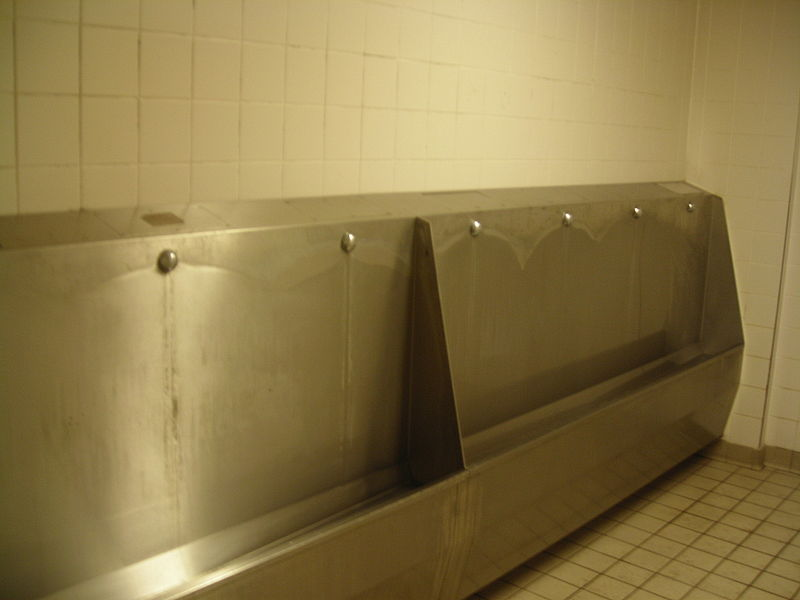
\includegraphics[width=0.6\textwidth]{sigbovik-urinal}}

\end{document}
